%!TEX root = memoria_duocode_interfaz.tex
\subsection{Base de datos}

A la vez que íbamos definiendo los requisitos, fuimos dándonos cuenta de las tablas y atributos que necesitaríamos en la base de datos y formamos el modelo entidad-relación (Figura \ref{fig:ent_rel}) y el modelo relacional (Figura \ref{fig:rel}).

\begin{sidewaysfigure}
\begin{center}
\makebox[\textwidth]{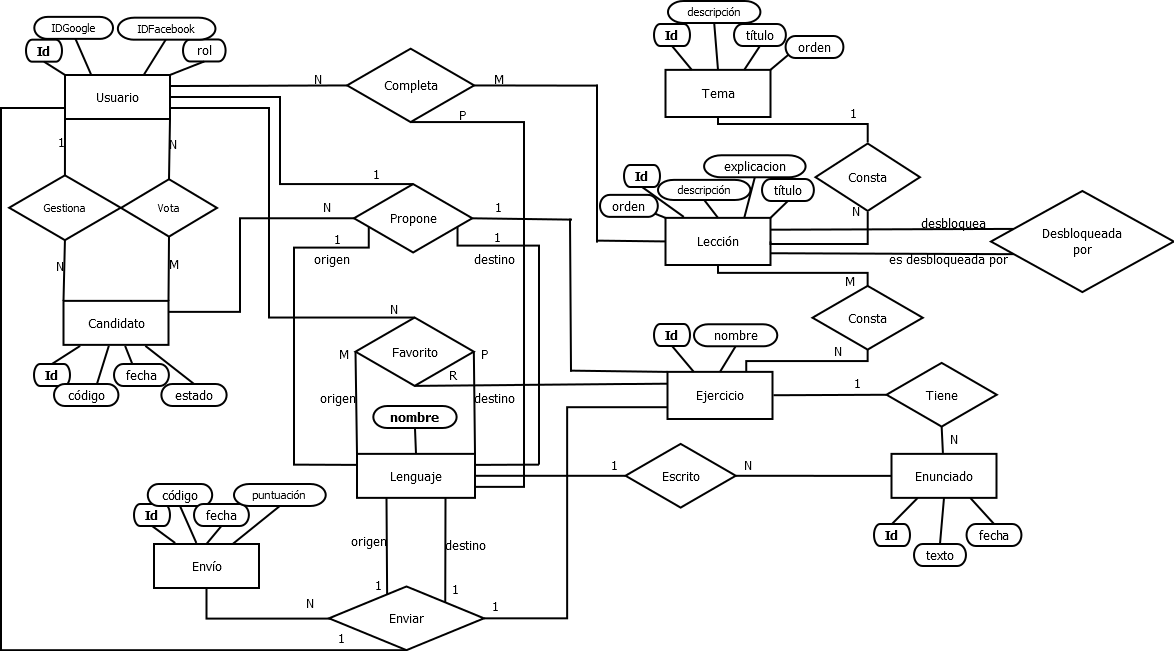
\includegraphics[width=\paperwidth]{images/bd-tfg}}
\caption{Modelo entidad-relacion\label{fig:ent_rel}}
\end{center}
\end{sidewaysfigure}

\begin{figure}
\begin{center}
\makebox[\textwidth]{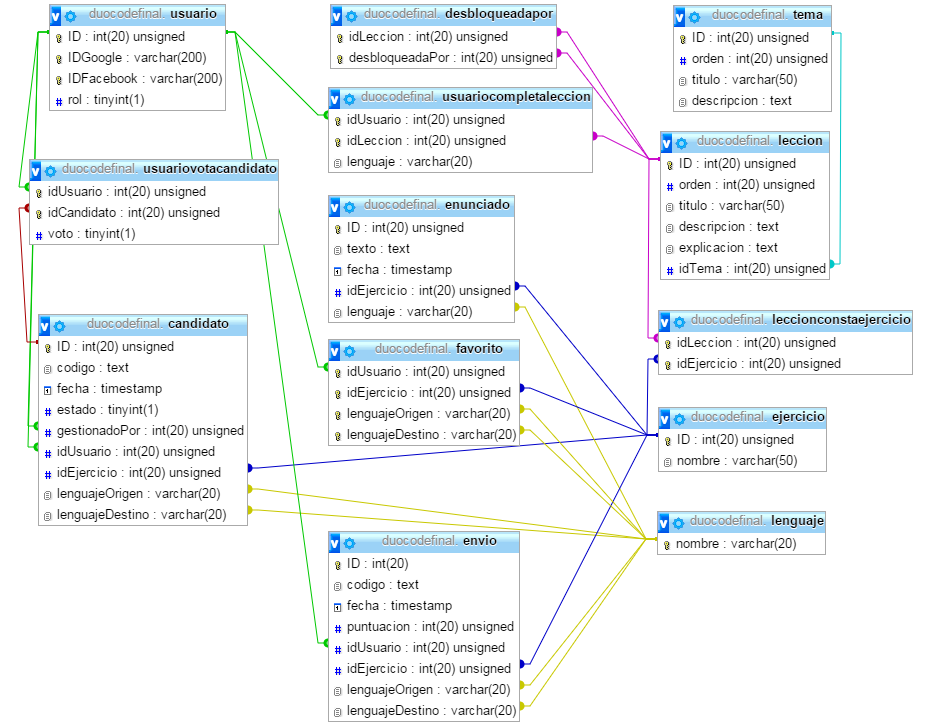
\includegraphics[scale=0.7]{images/bd}}
\caption{Modelo relacional\label{fig:rel}}
\end{center}
\end{figure}

\newpage

\textbf{Estructura de las tablas}

\begin{itemize}
\item Usuario: Tabla que contiene los datos de los usuarios. No hace falta guardar el nombre u otros datos personales ya que los obtenemos de la aplicación con la que haya iniciado sesión.


\begin{tabularx}{14cm}{|l|X|}
\hline
\textbf{Nombre} & \textbf{Descripción}                                                              \\ \hline
ID              & ID que le asigna la aplicación al usuario.                                         \\ \hline
IDGoogle        & ID que le asigna Google. Es opcional ya que el usuario puede iniciar con Facebook. \\ \hline
IDFacebook      & ID que le asigna Facebook. Es opcional ya que el usuario puede iniciar con Google. \\ \hline
\end{tabularx}
\vspace{1em}

\item UsuarioVotaCandidato: Tabla que contiene todos los votos de los usuarios a los candidatos.

\begin{tabularx}{14cm}{|l|X|}
\hline
\textbf{Nombre} & \textbf{Descripción}                                                              \\ \hline
IDUsuario       & ID del usuario que vota.                                                           \\ \hline
IDCandidato     & ID del candidato al que se quiere votar.                                           \\ \hline
Voto            & Puede tomar los valores 0 o 1 dependiendo de si el voto es positivo (1) o negativo (0). \\ \hline
\end{tabularx}
\vspace{1em}

\item Candidato: Tabla que contiene la información de los candidatos enviados por los usuarios de la aplicación.

\begin{tabularx}{14cm}{|l|X|}
\hline
\textbf{Nombre} & \textbf{Descripción}                                                              \\ \hline
ID              & Identificador único para el candidato.                                         \\ \hline
Código        & Texto propuesto como posible solución del ejercicio. \\ \hline
Fecha      & Fecha en la que se realiza la propuesta. \\ \hline
Estado              & Puede ser No Gestionado (0), Aceptado (1) o Rechazado (-1).                                         \\ \hline
GestionadoPor        & ID del usuario administrador que finalmente acepta o rechaza el candidato. Inicialmente se encuentra vacío. \\ \hline
IDUsuario      & ID del usuario que propone el candidato. \\ \hline
IDEjercicio              & ID del ejercicio que resuelve dicho candidato.                                         \\ \hline
LenguajeOrigen        & Lenguaje en el que se encuentra el enunciado del ejercicio. \\ \hline
LenguajeDestino      & Lenguaje en el que está la posible solución. \\ \hline
\end{tabularx}
\vspace{1em}

\item Tema: Tabla que contiene la información de los temas, primera división para organizar los ejercicios según a qué van dedicados. Los temas se conforman de una colección de lecciones.

\begin{tabularx}{14cm}{|l|X|}
\hline
\textbf{Nombre} & \textbf{Descripción}                                                              \\ \hline
ID       & ID propio del tema                                                           \\ \hline
Orden     & Orden en el que queremos que aparezca el tema.                                           \\ \hline
Título            & Nombre que distingue a los temas. \\ \hline
Descripción            & Texto breve que describe el tema. \\ \hline
\end{tabularx}
\vspace{1em}

\item Lección: Tabla que contiene la información de las lecciones, segunda división para la organización. Las lecciones se conforman de una serie de ejercicios y están incluidas en temas.

\begin{tabularx}{14cm}{|l|X|}
\hline
\textbf{Nombre} & \textbf{Descripción}                                                              \\ \hline
ID              & Identificador único para la lección.                                         \\ \hline
Orden        & Orden en el que queremos que aparezca la lección. \\ \hline
Título      & Nombre que distingue a las lecciones. \\ \hline
Descripción              & Texto breve que describe la lección.                                         \\ \hline
Expliciación        & Texto largo que sirve como introducción a la lección.  \\ \hline
IDTema      & ID del tema al que pertenece esta lección. \\ \hline
\end{tabularx}
\vspace{1em}

\item UsuarioCompletaLeccion: Tabla que contiene la relación de las lecciones con los usuarios que las han completado.

\begin{tabularx}{14cm}{|l|X|}
\hline
\textbf{Nombre} & \textbf{Descripción}                                                              \\ \hline
IDUsuario       & ID del usuario que ha completado la lección.                                                          \\ \hline
IDLección     & Lección que ha sido completada.                                           \\ \hline
Lenguaje            & Lenguaje en el que se ha completado dicha lección, ya que una lección puede ser completada por el mismo usuario en distintos lenguajes. \\ \hline
\end{tabularx}
\vspace{1em}

\item DesbloqueadaPor: Tabla que contiene la dependencia entre lecciones. Hay lecciones a las que solo se puede acceder si se han superado otras anteriormente.

\begin{tabularx}{14cm}{|l|X|}
\hline
\textbf{Nombre} & \textbf{Descripción}                                                              \\ \hline
IDLección       & ID de la lección a la que queremos asignar dependencia.                                                          \\ \hline
DesbloqueadaPor     & Lección que debe ser superada para poder acceder a la mencionada anteriormente.                                           \\ \hline
Lenguaje            & Lenguaje en el que se ha completado dicha lección, ya que una lección puede ser completada por el mismo usuario en distintos lenguajes. \\ \hline
\end{tabularx}
\vspace{1em}

\item Ejercicio: Tabla que contiene la información de los ejercicios existentes.

\begin{tabularx}{14cm}{|l|X|}
\hline
\textbf{Nombre} & \textbf{Descripción}                                                              \\ \hline
ID       & Identificador asignado por la aplicación para cada ejercicio. \\ \hline
Nombre     & Nombre con el que se diferenciará de los demás.                                           \\ \hline
\end{tabularx}
\vspace{1em}

\item LeccionConstaEjercicio: Tabla que contiene la relación donde se asignan los ejercicios a las correspondientes lecciones.

\begin{tabularx}{14cm}{|l|X|}
\hline
\textbf{Nombre} & \textbf{Descripción}                                                              \\ \hline
IDLección       & ID de la lección a la que se añade un ejercicio. \\ \hline
IDEjercicio     & ID del ejercicio añadido a la lección.                                           \\ \hline
\end{tabularx}
\vspace{1em}

\item Lenguaje: Tabla que contiene los lenguajes que podrán aprender los usuarios.

\begin{tabularx}{14cm}{|l|X|}
\hline
\textbf{Nombre} & \textbf{Descripción}                                                              \\ \hline
Nombre       & Nombre del lenguaje. \\ \hline
\end{tabularx}
\vspace{1em}

\item Enunciado: Tabla que contiene la información de los enunciados. Un enunciado es un código con un correspondiente lenguaje que forma parte de un ejercicio. Un ejercicio puede tener varios enunciados en varios idiomas.

\begin{tabularx}{14cm}{|l|X|}
\hline
\textbf{Nombre} & \textbf{Descripción}                                                              \\ \hline
ID       & ID que identifica al enunciado. \\ \hline
Texto     & Código, en lenguaje de origen, que tendrá que ser \emph{traducido}.                                           \\ \hline
Fecha     & Fecha en la que fue añadido el enunciado.                                           \\ \hline
IDEjercicio     & ID del ejercicio al que corresponde este enunciado.                                           \\ \hline
Lenguaje     & Lenguaje en el que está escrito el código de dicho enunciado.                                           \\ \hline
\end{tabularx}
\vspace{1em}

\item Favorito: Tabla que contiene la relación entre los usuarios y los ejercicios favoritos de estos.

\begin{tabularx}{14cm}{|l|X|}
\hline
\textbf{Nombre} & \textbf{Descripción}                                                              \\ \hline
IDUsuario       & ID del usuario que añade un ejercicio a favorito. \\ \hline
IDEjercicio     & ID del ejercicio que ha sido marcado como favorito. \emph{traducido}                                           \\ \hline
LenguajeOrigen     & Lenguaje del enunciado que ha sido marcado como favorito.                                           \\ \hline
LenguajeDestino     & Lenguaje que el usuario quería aprender al marcar este ejercicio como favorito.                                           \\ \hline
\end{tabularx}
\vspace{1em}

\item Envío: Tabla que contiene la relación entre los usuarios y todos los ejercicios que han realizado en la aplicación.

\begin{tabularx}{14cm}{|l|X|}
\hline
\textbf{Nombre} & \textbf{Descripción}                                                              \\ \hline
ID       & ID correspondiente a cada envío. \\ \hline
Código     & Código respuesta del usuario. \emph{traducido}                                           \\ \hline
Fecha     & Fecha en la que se ha resuelto el ejercicio.                                           \\ \hline
Puntuación     & Puntuación obtenida.                                           \\ \hline
IDUsuario     & Usuario que ha realizado el envío.                                           \\ \hline
IDEjercicio     & Ejercicio resuelto.                                           \\ \hline
LenguajeOrigen     & Lenguaje inicial del enunciado.                                           \\ \hline
LenguajeDestino     & Lenguaje en el que el usuario ha enviado el ejercicio.                                           \\ \hline
\end{tabularx}

\end{itemize}